% !TeX root = ./0Base.tex

\chapter{Criteria description}

\section{Performance benchmark}

\subsection{Scenarios}
The task for each application is to complete simple \acrshort{crud} operations as fast as possible. For comparison of the performance of the applications, a few test cases were developed:

\begin{itemize}
    \item retrieving multiple objects (getMany)
    \item retrieving single object (get)
    \item updating a single object (put)
    \item creating a single object (post)
    \item deleting a single object (delete)
\end{itemize}

They were tested with a few different application loads, which are represented by a number of \acrlong{vu}s (\acrshort{vu}s) - as mentioned in the k6 repository description they are glorified, parallel while(true) loops \cite{k6Git}.
The scenarios chosen for tests are:
\begin{itemize}
    \item 1 \acrshort{vu}
    \item 8 \acrshort{vu}s
    \item 32 \acrshort{vu}s
    \item 128 \acrshort{vu}s
    \item 512 \acrshort{vu}s
\end{itemize}
For a single virtual user case the number of concurrences does not change throughout the duration of the test, however, as suggested in
% TODO find article that suggests this
, for bigger numbers of concurrent users, the tests should include warmup and cooldown period. All tests are 45 seconds long, and tests with more than 1 virtual user include 15 seconds of ramp up time and 15 seconds of ramp down time as shown on figure \ref{fig:vusPerSecond}.

Longer test times did not bring any satisfactory results and only caused CPU throttling problems, thus they were shortened to the period of 45 total seconds, which also made comparison of the results much easier.

For one scenario the results could be slightly different, that is why every test was repeated 10 times. For creation of the graphs presented in chapter \ref{cha:results} for each test an average response times were calculated. 

\begin{figure}[H]
    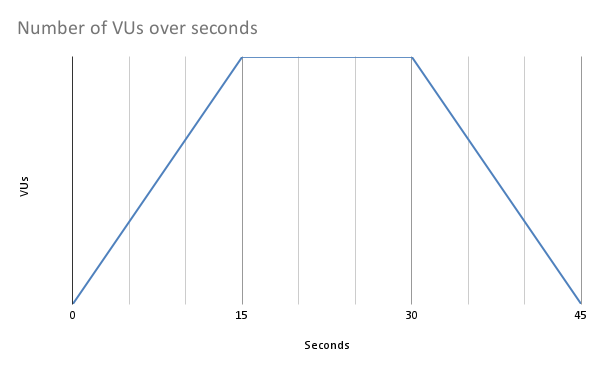
\includegraphics[width=\columnwidth]{pictures/vusPerSecond.png}
    \caption{Amount of VUs per second during the tests}
    \label{fig:vusPerSecond}
\end{figure}


\subsection{Data}

For the performance tests some frameworks required initial data to exist in the database (for example PUT endpoint for editing database models), thus at the beginning of the tests for each framework the database is populated. To be sure that the data is consistent, after seeding the database the docker volume that keeps the data is being stored locally, and before each test it is being restored.

\subsection{Application isolation}

To be sure that the applications are running in an isolated environment, docker containers were used. The configuration prepared for the applications included environment preparation (installing necessary packages, providing environment variables), To simplify the research, a Docker Compose configuration was prepared, that builds and starts all the necessary containers at once.

\subsection{Test progress}

The main script prepared for this thesis, that gathers all the measurements is described in the algorithm \ref{alg:testProgress}.

\begin{algorithm}[H]
    \label{alg:testProgress}
    \caption{Pseudocode describing load testing process}

    frameworks = [aspnet django express]\;
    scenarios = [1 8 32 128 512]\;
    iterations = [1 2 3 4 5 6 7 8 9 10]\;
    test cases = [get post put delete getMany]\;

    \ForAll{frameworks}{
        start application and database\;
        populate database\;
        kill application and database\;
        store snapshot\;
        \ForAll{scenarios}{
            \ForAll{iterations}{
                \ForAll{test cases}{
                    \If{application is running}{kill application and database\;}
                    remove volumes\;
                    \If{test case is not post}{restore snapshot\;}
                    start application and database\;
                    \While{application is not responding}{wait for application\;}
                    \For{45 seconds}{measured test\;}
                    store k6 result \;
                    store influxDB result \;
                    \For{20 seconds}{cooldown before next test\;}
                }
            }
        }
    }
    merge results\;
\end{algorithm}


\subsection{Software versions and hardware}

The tests were run on a laptop with the specification presented in table \ref{tab:hardware}.
Frameworks used to build the application were in the versions presented in table \ref{tab:software}.


\FloatBarrier
\begin{table}[!htp]\centering
    \caption{Hardware}\label{tab:hardware}
    \scriptsize
    \begin{tabular}{lrr}\toprule
        Hardware         &                                          \\\midrule
        Processor        & Intel(R) Core(TM) i5-8250U CPU @ 1.60GHz \\
        RAM memory       & 16 GB @ 2400MT/s                         \\
        Operating system & Ubuntu 20.04.2 LTS                       \\
        \bottomrule
    \end{tabular}
\end{table}
\FloatBarrier


\FloatBarrier
\begin{table}[!htp]\centering
    \caption{Frameworks and libraries versions}\label{tab:software}
    \scriptsize
    \begin{tabular}{lrr}\toprule
        Software versions                     &         \\\midrule
        Python                                & 3.1.9   \\
        Django                                & 3.1.4   \\
        Django REST Framework                 & 3.12.2  \\
        gunicorn                              & 20.0.4  \\
        uvicorn                               & 0.13.1  \\\midrule
        C\#                                   & 7.3     \\
        ASP.NET                               & 2.1.1   \\
        Npgsql.EntityFrameworkCore.PostgreSQL & 2.1.1.1 \\\midrule
        Node.js                               & 15.12.0 \\
        Express                               & 4.17.1  \\
        pg-promise                            & 10.9.5  \\
        body-parser                           & 1.19.0  \\
        \bottomrule
    \end{tabular}
\end{table}
\FloatBarrier


\section{Security}
